
%% bare_conf.tex
%% V1.4b
%% 2015/08/26
%% by Michael Shell
%% See:
%% http://www.michaelshell.org/
%% for current contact information.
%%
%% This is a skeleton file demonstrating the use of IEEEtran.cls
%% (requires IEEEtran.cls version 1.8b or later) with an IEEE
%% conference paper.
%%
%% Support sites:
%% http://www.michaelshell.org/tex/ieeetran/
%% http://www.ctan.org/pkg/ieeetran
%% and
%% http://www.ieee.org/

%%*************************************************************************
%% Legal Notice:
%% This code is offered as-is without any warranty either expressed or
%% implied; without even the implied warranty of MERCHANTABILITY or
%% FITNESS FOR A PARTICULAR PURPOSE!
%% User assumes all risk.
%% In no event shall the IEEE or any contributor to this code be liable for
%% any damages or losses, including, but not limited to, incidental,
%% consequential, or any other damages, resulting from the use or misuse
%% of any information contained here.
%%
%% All comments are the opinions of their respective authors and are not
%% necessarily endorsed by the IEEE.
%%
%% This work is distributed under the LaTeX Project Public License (LPPL)
%% ( http://www.latex-project.org/ ) version 1.3, and may be freely used,
%% distributed and modified. A copy of the LPPL, version 1.3, is included
%% in the base LaTeX documentation of all distributions of LaTeX released
%% 2003/12/01 or later.
%% Retain all contribution notices and credits.
%% ** Modified files should be clearly indicated as such, including  **
%% ** renaming them and changing author support contact information. **
%%*************************************************************************


% *** Authors should verify (and, if needed, correct) their LaTeX system  ***
% *** with the testflow diagnostic prior to trusting their LaTeX platform ***
% *** with production work. The IEEE's font choices and paper sizes can   ***
% *** trigger bugs that do not appear when using other class files.       ***                          ***
% The testflow support page is at:
% http://www.michaelshell.org/tex/testflow/

\documentclass[conference]{IEEEtran}
% Some Computer Society conferences also require the compsoc mode option,
% but others use the standard conference format.
%
% If IEEEtran.cls has not been installed into the LaTeX system files,
% manually specify the path to it like:
% \documentclass[conference]{../sty/IEEEtran}

% \usepackage[brazil]{babel}
% \usepackage[latin1]{inputenc}

\usepackage{graphicx,url}
\usepackage{float}
\usepackage{tikz}
\usetikzlibrary{shapes, arrows, shapes.geometric}

\usepackage[brazilian]{babel}
\usepackage[utf8]{inputenc}
\usepackage[T1]{fontenc}

\graphicspath{ {../images/} }

% \usepackage{tikz}
% \usetikzlibrary{shapes, arrows, shapes.geometric}


% Some very useful LaTeX packages include:
% (uncomment the ones you want to load)


% *** MISC UTILITY PACKAGES ***
%
%\usepackage{ifpdf}
% Heiko Oberdiek's ifpdf.sty is very useful if you need conditional
% compilation based on whether the output is pdf or dvi.
% usage:
% \ifpdf
%   % pdf code
% \else
%   % dvi code
% \fi
% The latest version of ifpdf.sty can be obtained from:
% http://www.ctan.org/pkg/ifpdf
% Also, note that IEEEtran.cls V1.7 and later provides a builtin
% \ifCLASSINFOpdf conditional that works the same way.
% When switching from latex to pdflatex and vice-versa, the compiler may
% have to be run twice to clear warning/error messages.






% *** CITATION PACKAGES ***
%
%\usepackage{cite}
% cite.sty was written by Donald Arseneau
% V1.6 and later of IEEEtran pre-defines the format of the cite.sty package
% \cite{} output to follow that of the IEEE. Loading the cite package will
% result in citation numbers being automatically sorted and properly
% "compressed/ranged". e.g., [1], [9], [2], [7], [5], [6] without using
% cite.sty will become [1], [2], [5]--[7], [9] using cite.sty. cite.sty's
% \cite will automatically add leading space, if needed. Use cite.sty's
% noadjust option (cite.sty V3.8 and later) if you want to turn this off
% such as if a citation ever needs to be enclosed in parenthesis.
% cite.sty is already installed on most LaTeX systems. Be sure and use
% version 5.0 (2009-03-20) and later if using hyperref.sty.
% The latest version can be obtained at:
% http://www.ctan.org/pkg/cite
% The documentation is contained in the cite.sty file itself.






% *** GRAPHICS RELATED PACKAGES ***
%
\ifCLASSINFOpdf
  % \usepackage[pdftex]{graphicx}
  % declare the path(s) where your graphic files are
  % \graphicspath{{../pdf/}{../jpeg/}}
  % and their extensions so you won't have to specify these with
  % every instance of \includegraphics
  % \DeclareGraphicsExtensions{.pdf,.jpeg,.png}
\else
  % or other class option (dvipsone, dvipdf, if not using dvips). graphicx
  % will default to the driver specified in the system graphics.cfg if no
  % driver is specified.
  % \usepackage[dvips]{graphicx}
  % declare the path(s) where your graphic files are
  % \graphicspath{{../eps/}}
  % and their extensions so you won't have to specify these with
  % every instance of \includegraphics
  % \DeclareGraphicsExtensions{.eps}
\fi
% graphicx was written by David Carlisle and Sebastian Rahtz. It is
% required if you want graphics, photos, etc. graphicx.sty is already
% installed on most LaTeX systems. The latest version and documentation
% can be obtained at:
% http://www.ctan.org/pkg/graphicx
% Another good source of documentation is "Using Imported Graphics in
% LaTeX2e" by Keith Reckdahl which can be found at:
% http://www.ctan.org/pkg/epslatex
%
% latex, and pdflatex in dvi mode, support graphics in encapsulated
% postscript (.eps) format. pdflatex in pdf mode supports graphics
% in .pdf, .jpeg, .png and .mps (metapost) formats. Users should ensure
% that all non-photo figures use a vector format (.eps, .pdf, .mps) and
% not a bitmapped formats (.jpeg, .png). The IEEE frowns on bitmapped formats
% which can result in "jaggedy"/blurry rendering of lines and letters as
% well as large increases in file sizes.
%
% You can find documentation about the pdfTeX application at:
% http://www.tug.org/applications/pdftex





% *** MATH PACKAGES ***
%
%\usepackage{amsmath}
% A popular package from the American Mathematical Society that provides
% many useful and powerful commands for dealing with mathematics.
%
% Note that the amsmath package sets \interdisplaylinepenalty to 10000
% thus preventing page breaks from occurring within multiline equations. Use:
%\interdisplaylinepenalty=2500
% after loading amsmath to restore such page breaks as IEEEtran.cls normally
% does. amsmath.sty is already installed on most LaTeX systems. The latest
% version and documentation can be obtained at:
% http://www.ctan.org/pkg/amsmath





% *** SPECIALIZED LIST PACKAGES ***
%
%\usepackage{algorithmic}
% algorithmic.sty was written by Peter Williams and Rogerio Brito.
% This package provides an algorithmic environment fo describing algorithms.
% You can use the algorithmic environment in-text or within a figure
% environment to provide for a floating algorithm. Do NOT use the algorithm
% floating environment provided by algorithm.sty (by the same authors) or
% algorithm2e.sty (by Christophe Fiorio) as the IEEE does not use dedicated
% algorithm float types and packages that provide these will not provide
% correct IEEE style captions. The latest version and documentation of
% algorithmic.sty can be obtained at:
% http://www.ctan.org/pkg/algorithms
% Also of interest may be the (relatively newer and more customizable)
% algorithmicx.sty package by Szasz Janos:
% http://www.ctan.org/pkg/algorithmicx




% *** ALIGNMENT PACKAGES ***
%
%\usepackage{array}
% Frank Mittelbach's and David Carlisle's array.sty patches and improves
% the standard LaTeX2e array and tabular environments to provide better
% appearance and additional user controls. As the default LaTeX2e table
% generation code is lacking to the point of almost being broken with
% respect to the quality of the end results, all users are strongly
% advised to use an enhanced (at the very least that provided by array.sty)
% set of table tools. array.sty is already installed on most systems. The
% latest version and documentation can be obtained at:
% http://www.ctan.org/pkg/array


% IEEEtran contains the IEEEeqnarray family of commands that can be used to
% generate multiline equations as well as matrices, tables, etc., of high
% quality.




% *** SUBFIGURE PACKAGES ***
%\ifCLASSOPTIONcompsoc
%  \usepackage[caption=false,font=normalsize,labelfont=sf,textfont=sf]{subfig}
%\else
%  \usepackage[caption=false,font=footnotesize]{subfig}
%\fi
% subfig.sty, written by Steven Douglas Cochran, is the modern replacement
% for subfigure.sty, the latter of which is no longer maintained and is
% incompatible with some LaTeX packages including fixltx2e. However,
% subfig.sty requires and automatically loads Axel Sommerfeldt's caption.sty
% which will override IEEEtran.cls' handling of captions and this will result
% in non-IEEE style figure/table captions. To prevent this problem, be sure
% and invoke subfig.sty's "caption=false" package option (available since
% subfig.sty version 1.3, 2005/06/28) as this is will preserve IEEEtran.cls
% handling of captions.
% Note that the Computer Society format requires a larger sans serif font
% than the serif footnote size font used in traditional IEEE formatting
% and thus the need to invoke different subfig.sty package options depending
% on whether compsoc mode has been enabled.
%
% The latest version and documentation of subfig.sty can be obtained at:
% http://www.ctan.org/pkg/subfig




% *** FLOAT PACKAGES ***
%
%\usepackage{fixltx2e}
% fixltx2e, the successor to the earlier fix2col.sty, was written by
% Frank Mittelbach and David Carlisle. This package corrects a few problems
% in the LaTeX2e kernel, the most notable of which is that in current
% LaTeX2e releases, the ordering of single and double column floats is not
% guaranteed to be preserved. Thus, an unpatched LaTeX2e can allow a
% single column figure to be placed prior to an earlier double column
% figure.
% Be aware that LaTeX2e kernels dated 2015 and later have fixltx2e.sty's
% corrections already built into the system in which case a warning will
% be issued if an attempt is made to load fixltx2e.sty as it is no longer
% needed.
% The latest version and documentation can be found at:
% http://www.ctan.org/pkg/fixltx2e


%\usepackage{stfloats}
% stfloats.sty was written by Sigitas Tolusis. This package gives LaTeX2e
% the ability to do double column floats at the bottom of the page as well
% as the top. (e.g., "\begin{figure*}[!b]" is not normally possible in
% LaTeX2e). It also provides a command:
%\fnbelowfloat
% to enable the placement of footnotes below bottom floats (the standard
% LaTeX2e kernel puts them above bottom floats). This is an invasive package
% which rewrites many portions of the LaTeX2e float routines. It may not work
% with other packages that modify the LaTeX2e float routines. The latest
% version and documentation can be obtained at:
% http://www.ctan.org/pkg/stfloats
% Do not use the stfloats baselinefloat ability as the IEEE does not allow
% \baselineskip to stretch. Authors submitting work to the IEEE should note
% that the IEEE rarely uses double column equations and that authors should try
% to avoid such use. Do not be tempted to use the cuted.sty or midfloat.sty
% packages (also by Sigitas Tolusis) as the IEEE does not format its papers in
% such ways.
% Do not attempt to use stfloats with fixltx2e as they are incompatible.
% Instead, use Morten Hogholm'a dblfloatfix which combines the features
% of both fixltx2e and stfloats:
%
% \usepackage{dblfloatfix}
% The latest version can be found at:
% http://www.ctan.org/pkg/dblfloatfix




% *** PDF, URL AND HYPERLINK PACKAGES ***
%
%\usepackage{url}
% url.sty was written by Donald Arseneau. It provides better support for
% handling and breaking URLs. url.sty is already installed on most LaTeX
% systems. The latest version and documentation can be obtained at:
% http://www.ctan.org/pkg/url
% Basically, \url{my_url_here}.




% *** Do not adjust lengths that control margins, column widths, etc. ***
% *** Do not use packages that alter fonts (such as pslatex).         ***
% There should be no need to do such things with IEEEtran.cls V1.6 and later.
% (Unless specifically asked to do so by the journal or conference you plan
% to submit to, of course. )


% correct bad hyphenation here
\hyphenation{op-tical net-works semi-conduc-tor}


\begin{document}
%
% paper title
% Titles are generally capitalized except for words such as a, an, and, as,
% at, but, by, for, in, nor, of, on, or, the, to and up, which are usually
% not capitalized unless they are the first or last word of the title.
% Linebreaks \\ can be used within to get better formatting as desired.
% Do not put math or special symbols in the title.
\title{VRSnake: um Jogo de Realidade Virtual em GPGPU}


% author names and affiliations
% use a multiple column layout for up to three different
% affiliations
% \author{Adriano M. Gil\inst{1}, Eliamara Silva\inst{1}, Thiago S. Figueira\inst{1}}

% \address{Samsung Instituto de Desenvolvimento para a Informática da Amazônia
%   (SIDIA)\\
%   Manaus -- AM -- Brazil
%   \email{\{adriano.gil,eliamara.s,t.figueira\}@samsung.com}
% }

\author{\IEEEauthorblockN{Thiago S. Figueira\IEEEauthorrefmark{1},
Adriano M. Gil\IEEEauthorrefmark{1}}
\IEEEauthorblockA{\IEEEauthorrefmark{1}Samsung Instituto de Desenvolvimento para a Informática da Amazônia\\
SIDIA,\\
Manaus -- AM -- Brazil}}

% conference papers do not typically use \thanks and this command
% is locked out in conference mode. If really needed, such as for
% the acknowledgment of grants, issue a \IEEEoverridecommandlockouts
% after \documentclass

% for over three affiliations, or if they all won't fit within the width
% of the page, use this alternative format:
%
%\author{\IEEEauthorblockN{Michael Shell\IEEEauthorrefmark{1},
%Homer Simpson\IEEEauthorrefmark{2},
%James Kirk\IEEEauthorrefmark{3},
%Montgomery Scott\IEEEauthorrefmark{3} and
%Eldon Tyrell\IEEEauthorrefmark{4}}
%\IEEEauthorblockA{\IEEEauthorrefmark{1}School of Electrical and Computer Engineering\\
%Georgia Institute of Technology,
%Atlanta, Georgia 30332--0250\\ Email: see http://www.michaelshell.org/contact.html}
%\IEEEauthorblockA{\IEEEauthorrefmark{2}Twentieth Century Fox, Springfield, USA\\
%Email: homer@thesimpsons.com}
%\IEEEauthorblockA{\IEEEauthorrefmark{3}Starfleet Academy, San Francisco, California 96678-2391\\
%Telephone: (800) 555--1212, Fax: (888) 555--1212}
%\IEEEauthorblockA{\IEEEauthorrefmark{4}Tyrell Inc., 123 Replicant Street, Los Angeles, California 90210--4321}}




% use for special paper notices
%\IEEEspecialpapernotice{(Invited Paper)}




% make the title area
\maketitle

% As a general rule, do not put math, special symbols or citations
% in the abstract
\begin{abstract}
Aplicações de realidade virtual são caracterizadas pela alta sensibilidade à atrasos na sincronização entre os movimentos do usuário e a respectiva renderização do mundo virtual. Uma forma de acelerar a execução da camada lógica é transportar sua implementação para GPU.  Este artigo propõe uma arquitetura de visualização baseada em um shader parametrizado pelo variavéis de estados e movimentações dos elementos de jogo. Como exemplo dessa abordagem, implementamos uma versão do clássico jogo Snake onde todos os elementos visuais são definidos e desenhados via shader em um único \textit{Mesh}. Ao mesmo tempo, abordar-se a implementação do filtro de Kalman como forma de aprimorar o reconhecimento de sinais do controle de realidade virtual \textit{Gear VR Controller}.
\end{abstract}

% no keywords




% For peer review papers, you can put extra information on the cover
% page as needed:
% \ifCLASSOPTIONpeerreview
% \begin{center} \bfseries EDICS Category: 3-BBND \end{center}
% \fi
%
% For peerreview papers, this IEEEtran command inserts a page break and
% creates the second title. It will be ignored for other modes.
\IEEEpeerreviewmaketitle



\section{Introdução} \label{sec:introduction}
% Contextualizar a Unity
Para o desenvolvimento de aplicações VR, o motor e editor gráfico \textit{Unity} situa-se como peça de extrema relevância dadas a sua facilidade de aprendizado e simplicidade no processo de desenvolvimento, além da possibilidade de criação de jogos e aplicações para consoles, plataformas móveis e dispositivos de realidade virtual e realidade aumentada.

Normalmente, estes jogos e aplicações desenvolvidos na \textit{Unity} são compostos por conjuntos de cenas, cada qual com seu próprio agrupamento de objetos e lógica associados. De maneira geral, a CPU (\textit{central processing unit}) é responsável por transmitir informações sobre elementos gráficos à GPU (\textit{graphics processing unit}) através do estágio de aplicação, onde os \textit{assets} gráficos como modelos 3D e texturas são carregados na VRAM (\textit{video RAM}), posteriormente durante o estágio de geometria, os diferentes objetos que devem ser renderizados bem como seus respectivos posicionamentos e demais informes visuais relevantes são tratados pela GPU e convertidos em imagem, no estágio de rasterização \cite{akenine2008real}.

% Contextualizar a Realidade Virtual e Controladores
Em outro âmbito, os controles ou \textit{joysticks} são uma das formas de interação com dispositivos de realidade virtual, no entanto, são passíveis de ruídos devido à presença de sensores baseados em magnetômetros, originando comportamentos indesejados como \textit{jittering} durante a leitura dos dados.

% Resumo proposta
Neste trabalho, propomos o desenvolvimento de um jogo cujas representações gráficas sejam inteiramente fundamentadas em código de GPU ao passo que as restrições lógicas concentrem-se na CPU, de maneira a atuar nos diferentes estágios da \textit{pipeline} gráfica acima apresentada. Em alusão à um clássico, o jogo Snake será recriado para os dispositivos de realidade virtual da Samsung em uma aplicação Unity, diferencia-se, porém, na medida que o jogador controla o objeto coletável, posicionando-o com o controlador tendo a finalidade de fazer a serpente falhar em seu objetivo. Tendo em vista solucionar o primeiro desafio acima exposto intenta-se a aplicação do filtro de Kalman durante a leitura do posicionamento do cursor através deste \textit{joystick}, a fim de melhorar o reconhecimento do sinal e atenuar a inconsistência apresentada.

% * Estrutura do artigo
Analisamos na seção \ref{sec:relatedworks} outros trabalhos que abordam sensores, uso de filtros e jogos de realidade virtual. Um esclarecimento sobre as regras do jogo desenvolvido pode ser encontrado na seção \ref{sec:vrsnake}. A arquitetura proposta é detalhada na seção \ref{sec:architecture}. Apresenta-se como um jogo de realidade virtual pode ser renderizado em uma esfera invertida na seção \ref{sec:invertedsphere}. Em \ref{sec:agent}, comprende-se a movimentação da \textit{snake} e sua arquitetura de renderização. A seção \ref{sec:gearvrcontroller} explana como ocorre a aplicação do filtro de Kalman no controle para VR. Resultados são discutidos na seção \ref{sec:results}. Por fim, pautam-se as conclusões e perspectivas de trabalhos futuros na seção \ref{sec:conclusion}.


% An example of a floating figure using the graphicx package.
% Note that \label must occur AFTER (or within) \caption.
% For figures, \caption should occur after the \includegraphics.
% Note that IEEEtran v1.7 and later has special internal code that
% is designed to preserve the operation of \label within \caption
% even when the captionsoff option is in effect. However, because
% of issues like this, it may be the safest practice to put all your
% \label just after \caption rather than within \caption{}.
%
% Reminder: the "draftcls" or "draftclsnofoot", not "draft", class
% option should be used if it is desired that the figures are to be
% displayed while in draft mode.
%
%\begin{figure}[!t]
%\centering
%\includegraphics[width=2.5in]{myfigure}
% where an .eps filename suffix will be assumed under latex,
% and a .pdf suffix will be assumed for pdflatex; or what has been declared
% via \DeclareGraphicsExtensions.
%\caption{Simulation results for the network.}
%\label{fig_sim}
%\end{figure}

% Note that the IEEE typically puts floats only at the top, even when this
% results in a large percentage of a column being occupied by floats.


% An example of a double column floating figure using two subfigures.
% (The subfig.sty package must be loaded for this to work.)
% The subfigure \label commands are set within each subfloat command,
% and the \label for the overall figure must come after \caption.
% \hfil is used as a separator to get equal spacing.
% Watch out that the combined width of all the subfigures on a
% line do not exceed the text width or a line break will occur.
%
%\begin{figure*}[!t]
%\centering
%\subfloat[Case I]{\includegraphics[width=2.5in]{box}%
%\label{fig_first_case}}
%\hfil
%\subfloat[Case II]{\includegraphics[width=2.5in]{box}%
%\label{fig_second_case}}
%\caption{Simulation results for the network.}
%\label{fig_sim}
%\end{figure*}
%
% Note that often IEEE papers with subfigures do not employ subfigure
% captions (using the optional argument to \subfloat[]), but instead will
% reference/describe all of them (a), (b), etc., within the main caption.
% Be aware that for subfig.sty to generate the (a), (b), etc., subfigure
% labels, the optional argument to \subfloat must be present. If a
% subcaption is not desired, just leave its contents blank,
% e.g., \subfloat[].


% An example of a floating table. Note that, for IEEE style tables, the
% \caption command should come BEFORE the table and, given that table
% captions serve much like titles, are usually capitalized except for words
% such as a, an, and, as, at, but, by, for, in, nor, of, on, or, the, to
% and up, which are usually not capitalized unless they are the first or
% last word of the caption. Table text will default to \footnotesize as
% the IEEE normally uses this smaller font for tables.
% The \label must come after \caption as always.
%
%\begin{table}[!t]
%% increase table row spacing, adjust to taste
%\renewcommand{\arraystretch}{1.3}
% if using array.sty, it might be a good idea to tweak the value of
% \extrarowheight as needed to properly center the text within the cells
%\caption{An Example of a Table}
%\label{table_example}
%\centering
%% Some packages, such as MDW tools, offer better commands for making tables
%% than the plain LaTeX2e tabular which is used here.
%\begin{tabular}{|c||c|}
%\hline
%One & Two\\
%\hline
%Three & Four\\
%\hline
%\end{tabular}
%\end{table}


% Note that the IEEE does not put floats in the very first column
% - or typically anywhere on the first page for that matter. Also,
% in-text middle ("here") positioning is typically not used, but it
% is allowed and encouraged for Computer Society conferences (but
% not Computer Society journals). Most IEEE journals/conferences use
% top floats exclusively.
% Note that, LaTeX2e, unlike IEEE journals/conferences, places
% footnotes above bottom floats. This can be corrected via the
% \fnbelowfloat command of the stfloats package.



\section{Trabalhos Relacionados} \label{sec:relatedworks}

% TODO: Refrasear texto
O jogo bidimensional \textit{Jelly in the Sky}, recentemente disponibilizado para aquisição na plataforma de jogos para computador \textit{Steam}, utiliza uma estrutura baseada em \textit{shader} similar à arquitetura apresentada aqui. \cite{GPGPUWars} defendem um trabalho onde a GPU executa todo o processamento do jogo criado.

% TODO: Refrasear texto
 Contudo, aplicações em realidade virtual diferem de outras aplicações devido à necessidade de preencher o espaço tridimensional de forma a fornecer conteúdo para 3 graus de liberdade(3DoF - \textit{3 Degrees of Freedom}) possibilitados durante a construção deste trabalho. Por exemplo, a aplicação descrita em \cite{zund2015unfolding} utiliza visão computacional para geração de uma visão panorâmica de um jogo de console em 8-bits. Rodando em um Oculus Rift DK2, o jogador é posicionado no centro do mundo e à medida que movimenta seu personagem, o mundo se desdobra ao seu redor, extendendo a visão de jogo para as quatro paredes do ambiente virtual.

% 3 - Controles de VR auxiliam na sensação de presença e por consequência na imersão
% TODO: Refrasear texto
Jogos VR são um grande potencializador de imersão, dada a sua capacidade de estimular a sensação de presença espacial e interatividade \cite{seibert2017control} através, por exemplo, dos controles VR, tal qual o modelo ET-YO32 da Samsung exibido na figura \ref{fig:vrcontroller}, que são classificados como de mapeamento natural tangível realístico e consoante a definição proposta por \cite{skalski2011mapping}, emulam de forma realista sua contrapartida no ambiente virtual, ou seja, movimenta-se a réplica do controle físico no espaço 3D da aplicação VR da mesma forma que se faz no mundo real.

% 4 - Exemplos de filtragem de açoes dos controles (From ERIN17 paper. Refrasear)
% TODO: Refrasear texto
Certos trabalhos trazem a filtragem de sensores baseados no uso de acelerômetro, a exemplo: \cite{schlomer2008gesture} usa o modelo oculto de Markov para reconhecimento de gestos em um controle do \textit{Nintendo Wii}, a filtragem ocorre por meio de filtros simples para remover pontos que não são suficientemente expressivos. \cite{shiratori2008accelerometer}, por outro lado, utilizam múltiplos controles de \textit{Nintendo Wii} para gerar animações proceduralmente, o ruído é atenuado através do uso do filtro de Kalman.


%Reescrito
\section{VRSnake: Design do Jogo} \label{sec:vrsnake}
O \textit{VRSnake} é a versão em realidade virtual do clássico jogo 2D \textit{Snake}, que faz uso da unidade gráfica de processamento para calcular e renderizar um número expressivamente maior de elementos em tela quando comparado à sua contrapartida em CPU. 

* Aqui entram os comparativos graficos da CPU e GPU*

No jogo original controlava-se a serpente na busca pelos coletáveis distribuídos pelo cenário, o \textit{VRSnake} permite ao jogador controlar o posicionamento destes objetos coletáveis, desta forma seu principal objetivo é derrotar as diversas serpentes que estão espalhadas no universo virtual. Propomos então as regras como seguem:

As serpentes buscam ininterruptamente o objeto coletável posicionado pelo jogador e seguem até o objeto pelo percurso que as manterão vivas por mais tempo, isto é, as serpentes desviam de si mesmas e das demais serpentes quando possível. Se este desvio não acontece, uma das serpentes é eliminada. Em outro aspecto, caso o objeto coletável seja capturado com sucesso, a \textit{snake} cresce em uma unidade de medida. O jogador vence a partida quando resta unicamente uma serpente.

%Reescrevendo
\section{Arquitetura de um Jogo GPGPU}
Jogos são aplicações interativas que executam três classes de ações: coleta, processamento e exibição de dados. %Arranjar referencia sobre software (algo mais abrangente) 
A coleta de dados foca em recolher dados dos dispositivos de entrada sejam eles teclado, mouse, toque ou \textit{joysticks}. O processamento abrange o reconhecimento dos dados coletados e sua devida tradução para o mundo do jogo, mas também garante o cumprimento das regras e gerenciamento do estado geral da aplicação. A exibição é o passo final, pois retorna ao jogador as consequências de seus atos de maneira sensorial. Desta forma, o \textit{VRSnake} é um jogo de realidade virtual que concentra as ações das classes de processamento e exibição na unidade gráfica de processamento (GPU - \textit{Graphics Processing Unit}). 

Esta arquitetura foi implementada utilizando o motor gráfico \textit{Unity} através do HLSL (\textit{High Level Shading Language}) para os \textit{shaders} e CSharp como linguagem de programação de CPU (\textit{Central Processing Unit}).

%A arquitetura do \textit{VRSnake} é baseada em dois níveis. O primeiro nível é de responsabilidade da CPU e coleta os dados de entrada, o segundo nível envolve a GPU e o processamen


Propomos uma arquitetura de duas camadas respectivamente responsáveis pelo gerenciamento lógico e visualização (ou renderização) da aplicação. A primeira fora desenvolvida em \textit{csharp}, portanto executada na unidade central de processamento (CPU, em inglês) e encarregada das tarefas inteligentes tais como a procura pelo objeto coletável e movimentação, além da aplicação do filtro de Kalman durante a leitura de dados do controle.

A segunda camada envolve um \textit{shader}, código executado diretamente na unidade de processamento gráfico (GPU, em inglês), incumbido de renderizar todos os itens apresentados no dispositivo de saída, que incluem o plano de fundo, o objeto coletável circular bem como os quadriláteros que representam o personagem ou a \textit{snake}.

O diagrama abaixo ilustra, de maneira geral, o funcionamento da arquitetura. Fundamentalmente, a camada lógica gerencia a colisão e movimentação da \textit{snake}; seleciona o caminho mais promissor acrescido de um fator randômico; além de efetivamente aplicar o filtro de Kalman às entradas do controle. A camada de visualização, por outro lado, é responsável pela renderização de todos os elementos dispostos no dispositivo de saída, isto é, a CPU não tem responsabilidade sobre estes objetos.

\begin{figure}[H]
\centering
\tikzstyle{arrow} = [draw, -latex]
\begin{tikzpicture} [x=1.2cm, y=1cm, node distance=0,outer sep=0,inner sep=0]
    \draw (0, 0) rectangle (12,5);
    \draw[dashed] (6,0) -- (6,5);

    \draw (0,4.5) rectangle (6,5) node[pos=.5] {\small Camada Lógica (CSharp)};
    \draw (6, 4.5) rectangle (12, 5) node[pos=.5] {\small Camada de Visualização (Shader)};

    \draw (0.3, 3.7) rectangle (4, 4.2) node[pos=.5] (1A) {\small Gerenciamento de Colisão};
    \draw (0.6, 2.9) rectangle (4.6, 3.4) node[pos=.5] (2A) {\small Movimentação da Serpente};
    \draw (7, 2.9) rectangle (11, 3.4)node[pos=.5] (3A) {\small Renderização da Serpente};

    \draw (0.3, 2) rectangle (4.3, 2.5) node[pos=.5] (4A) {\small Aplicação do filtro de Kalman};
    \draw (0.4, 1.2) rectangle (5.8, 1.7) node[pos=.5] (5A) {\small Cálculo da Geometria do Plano de Fundo};
    \draw (7, 1.2) rectangle (11.7, 1.7) node[pos=.5] (6A) {\small Renderização do Plano de Fundo};

    \draw (0.3, 0.2) rectangle (5.9, 0.7) node[pos=.5] (7A) {\small Inteligência de Movimentação da Serpente};

    \path [arrow] (1A) -- (2A);
    \path [arrow] (2A) -- (3A);

    \path [arrow] (4A) -- (5A);
    \path [arrow] (5A) -- (6A);
\end{tikzpicture}
\caption{Diagrama de arquitetura da aplicação}
\label{fig:diagramaArquitetura}
\end{figure}


\section{VRSnake: Um agente inteligente}

A inteligência de movimentação da \textit{snake} é, por sua vez, composta por uma função utilitária de avaliação de estados que analisa cada possível ação em determinado momento. Em essência, a serpente sempre está buscando alcançar o coletável, por isso avalia o curso de menor distância no eixos X e Y e desde que não exista a possibilidade de atingir a si própria, assume este caminho e repete o processo. A função abaixo ilustra esse procedimento:

\begin{equation}
F(A) = R * (D + O)
\label{equation11}
\end{equation}

Onde R é um fator de randomização; D representa a distância de \textit{Manhattan} entre a posição atual e o objeto coletável; e O é um valor atribuído à existência ou não de obstáculos neste trajeto.

Para cada direção plausível apresentada na figura \ref{fig:snakeHeadPositions} abaixo, a função retorna um valor de utilidade que é ulteriormente comparado para determinar o caminho de maior probabilidade de sucesso.

A lógica de movimentação consiste em gerenciar o posicionamento da cabeça e corpo da serpente.  Em outras palavras, a cabeça norteia todo o movimentar da \textit{snake}, pois nela são traçados os vetores responsáveis por orientar a serpente na decisão do menor caminho entre sua atual posição e o objeto coletável. É relevante explicitar que estes vetores de direcionamento são volúveis tendo em vista as diferentes posições adotáveis, conforme a figura \ref{fig:snakeHeadPositions} abaixo, onde a seta em vermelho indica a atual orientação da serpente e as demais indicam possíveis direções de movimento.

O corpo da serpente, por sua vez, move-se através de um buffer deslizante: cada parte do corpo assume a posição mais recente da parte imediatamente anterior, isso significa que a cabeça move-se e as demais partes seguem posteriormente.

\begin{figure}[H]
\centering
\tikzstyle{arrow} = [draw, -latex]

\begin{tikzpicture} [x=1.2cm, y=1cm, node distance=0,outer sep=0,inner sep=0]
  \draw (0, 0) rectangle (1, 1) node[pos=.5] {\small Head};
  \draw (3, 0) rectangle (4, 1) node[pos=.5] {\small Head};
  \draw (6, 0) rectangle (7, 1) node[pos=.5] {\small Head};
  \draw (9, 0) rectangle (10, 1) node[pos=.5] {\small Head};

  \path [arrow, red] (0.5, 1) -- (0.5, 1.5);
  \path [arrow] (1, 0.5) -- (1.5, 0.5);
  \path [arrow] (0, 0.5) -- (-0.5, 0.5);

  \path [arrow, red] (3.5, 0) -- (3.5, -0.5);
  \path [arrow] (4, 0.5) -- (4.5, 0.5);
  \path [arrow] (3, 0.5) -- (2.5, 0.5);

  \path [arrow] (6.5, 1) -- (6.5, 1.5);
  \path [arrow, red] (7, 0.5) -- (7.5, 0.5);
  \path [arrow] (6.5, 0) -- (6.5, -0.5);

    \path [arrow] (9.5, 1) -- (9.5, 1.5);
  \path [arrow, red] (9, 0.5) -- (8.5, 0.5);
  \path [arrow] (9.5, 0) -- (9.5, -0.5);

\end{tikzpicture}
\caption{Possíveis movimentos da serpente, as setas coloridas indicam a direção atual}
\label{fig:snakeHeadPositions}
\end{figure}

Considerando ainda a restrição de deslocamento na qual a serpente pode-se mover unicamente nas direções apontadas pela figura \ref{fig:snakeHeadPositions}, o cálculo por meio da distância de Manhattan se mostrou menos custoso, uma vez que sua equação representada abaixo não envolve operações quadráticas as quais, no escopo desta aplicação, podem ser chamadas inúmeras vezes por segundo.

\begin{equation}
EuclidianDistance = \sqrt{(x_{1} - x_{2})^2 + (y_{1} - y_{2})^2}
\label{equation:euclidian}
\end{equation}

\begin{equation}
ManhattanDistance = \left|x_{1} - x_{2}\right| + \left|y_{1} - y_{2}\right|
\label{equation:manhattan}
\end{equation}

No que concerne a segunda camada, o \textit{shader} de renderização analisa durante a execução do jogo cada pixel para determinar a que elemento este pertence: o objeto coletável, a serpente ou o plano de fundo. Para determinar esta relação de atribuição, alguns cálculos básicos são necessários: um pixel é colorido com a cor do objeto coletável se sua distância até o centro do objeto (um pixel) for menor que um raio determinado, semelhantemente mantem-se um vetor de pontos equidistantes entre si, onde cada posição representa um quadrilátero que faz parte do corpo da \textit{snake}, o pixel em questão recebe a cor da serpente caso esteja contido na área delineada por estes quadriláteros, dados seus tamanhos de lado e centro, no entanto, uma vez que não atenda a nenhum caso anterior, o pixel simplesmente recebe a cor do plano de fundo.

Para que a serpente mova-se de forma circular deve-se compreender o mapeamento UV (projeção de uma imagem 2D em uma superfície 3D) da superfície do objeto, neste caso, uma esfera. Basta verificar as extremidades para a presença da \textit{snake} e redesenhá-la no lado apropriado.

\section{Realidade Virtual}

% 1 - O uso de uma esfera invertida para renderizar o conteúdo do jogo
% Imersão -> Preenchimento/Renderização de conteúdo ao redor do usuário
% TODO: Refrasear texto
A ilusão em um mundo virtual e consequente sensação de imersão requerem material visual disponível em todos os ângulos possíveis, uma vez que o gearVR possibilita completa liberdade de rotação, ou seja, 3 graus de liberdade (3DoF - \textit{3 Degrees of Freedom}). Tendo em vista que a proposta deste artigo contempla um jogo essencialmente 2D, tal como o \textit{Snake} original, tem-se o desafio de exibir conteúdo bidimensional em um cenário 3D de forma que tudo aconteça ao redor do usuário.

% TODO: Refrasear texto
Uma esfera invertida, ou seja, uma esfera que tenha apenas seu lado interno renderizado, possibilita preencher completamente todo o campo de visão possível, além de ser a solução padrão adotada na exibição de imagens equiretangulares em 360 graus. A geração procedural de uma esfera pode seguir uma das duas abordagens abaixo:
\begin{enumerate}
  \begin{item} uma icosfera, i.e. uma esfera cujos vértices são distribuídos uniformemente; \end{item}
  \begin{item} geração de vertíces baseada em coordenadas de longitude/latitude. \end{item}
\end{enumerate}

% TODO: Refrasear texto
Para este trabalho, preferiu-se a segunda abordagem devido a possibilidade de usar a longitude/latitude como forma de mapear as coordenadas de UV, através da conversão abaixo:

% TODO: Refrasear texto
O formato de imagem equiretangular é uma captura ou produção de imagem feita para ser exibida no interior de uma esfera possibilitando preencher completamente o campo de visão do usuário, além de ser a solução muito utilizada na exibição de imagens equiretangulares em 360 graus. O mapeamento de UV da esfera é o padrão adotado para \textit{softwares} de modelagem na geração de uma esfera: geração de vertíces baseada em coordenadas de longitude/latitude.

% \begin{figure}[!tbp]
%   \centering
%   \begin{minipage}[b]{0.40\textwidth}
%     \includegraphics[width=1.4\textwidth]{../images/equirect_projection.jpg}
%     \caption{Imagem 360 em formato equiretangular.}
%     \label{fig:equirectimage}
%   \end{minipage}
%   \hfill
%   \begin{minipage}[b]{0.44\textwidth}
%     \centering
%     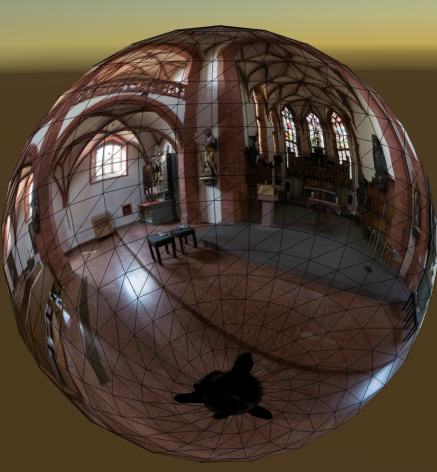
\includegraphics[width=0.7\textwidth]{../images/sphere.png}
%     \caption{Mapeamento de UV de uma imagem equiretangular para uma esfera.}
%     \label{fig:equisphere}
%   \end{minipage}
% \end{figure}

% 2 - Mapeamento de UV em uma esfera invertida
% Na figura \ref{fig:sphere_transversalsec} é exibida uma secção transversal da divisão de uma esfera em longitudes.
Na geração das posições dos vértices da esfera, se faz necessário definir uma quantidade de valores de longitude $N$, assim o tamanho angular $T$ para divisão longitudinal pode ser calculado pela equação \ref{longitudesize}.

% \begin{figure}[ht]
% \centering
% 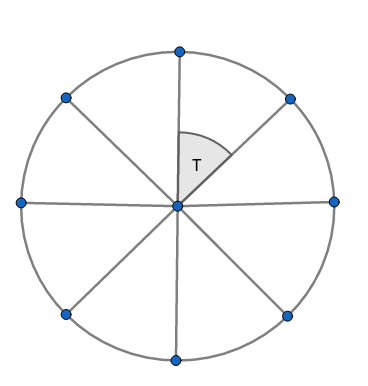
\includegraphics[width=.25\textwidth]{../images/longitudes.png}
% \caption{Uma secção transversal da esfera dividida em 8 longitudes.}
% \label{fig:sphere_transversalsec}
% \end{figure}

\begin{equation}
T = \frac{2 \pi}{N}
\label{longitudesize}
\end{equation}

O tamanho angular total de uma quantidade de $i$ de valores de longitude pode ser dada pela equação \ref{longitudealpha}.

\begin{equation}
\alpha_{i} = i * T
\label{longitudealpha}
\end{equation}

% Considerando a figura \ref{fig:sphere_transversalsec}, percebe-se que
O seno e cosseno do ângulo T definem-se as posições X e Z dos pontos da esfera pertencentes a essa secção transversal da esfera. Dessa forma, supondo uma esfera de raio $R$, podemos escrever as equações \ref{x_d} e \ref{z_d}.

\begin{equation}
x_{i} = R * \sin(\alpha_{i})
\label{x_d}
\end{equation}

\begin{equation}
z_{i} = R * \cos(\alpha_{i})
\label{z_d}
\end{equation}

Em um corte longitudinal, é possível perceber que o raio $R$ de uma secção transversal varia ao longo da altura da esfera. Determina-se então um valor $K$ como o tamanho angular de um valor de latitude da esfera, dado um valor $M$ de latitudes, tal como visto na equação \ref{equation5}.

% \begin{figure}[ht]
% \centering
% 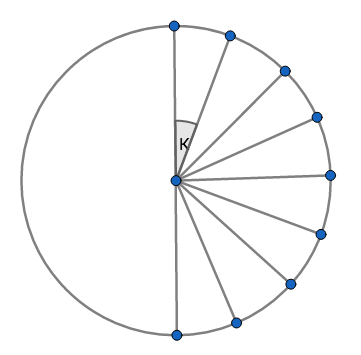
\includegraphics[width=.25\textwidth]{../images/latitudes.png}
% \caption{Uma secção longitudinal da esfera dividida em 8 latitudes.}
% \label{fig:sphere_longitudisec}
% \end{figure}

\begin{equation}
K = \frac{\pi}{M}
\label{equation5}
\end{equation}

O tamanho angular total de uma quantidade de $i$ de valores de latitude pode ser dado pela equação \ref{equation6}.

\begin{equation}
\alpha_{yi} = i * K
\label{equation6}
\end{equation}

A posição Y dos pontos da esfera, considerando raio unitário, pode ser dada pela equação \ref{equation7}.
\begin{equation}
y_{i} = \cos(\alpha_{yi})
\label{equation7}
\end{equation}

O raio $D_{yi}$ obtido em uma secção transversal na latitude $i$ é definido na equação \ref{equation8} como:
\begin{equation}
R_{yi} = \sin(\alpha_{yi})
\label{equation8}
\end{equation}

Aplicando-se a equação \ref{equation8} nas equações \ref{x_d} e \ref{z_d} obtém-se as posições X e Z dos vértices da esfera em função de suas coordenadas de longitude e latitude.

\begin{equation}
x_{i} = \sin(\alpha_{yi}) * \sin(\alpha_i)
\label{equation9}
\end{equation}

\begin{equation}
z_{i} = \sin(\alpha_{yi}) * \cos(\alpha_i)
\label{equation10}
\end{equation}


\subsection{Uso do Controle VR com Filtro de Kalman} \label{sec:gearvrcontroller}
Devido à natureza do jogo desenvolvido, o jogador necessita controlar o posicionamento do objeto coletável e para tanto existem essencialmente duas formas de interação num dispositivo de realidade virtual: o HMD (\textit{head-mounted display}), ou seja, através do sensor lateral acoplado ao próprio dispositivo; e os controladores externos, como os controles ou \textit{joysticks}. Em sua condição de sensor, porém, estes controladores estão sujeitos à interferência ruidosa durante a virtualização do evento representado no mundo real pelo movimento do usuário. Com a finalidade de melhorar a captura do sinal e traduzir de maneira mais fiel as intenções do jogador, o filtro de Kalman será aplicado às leituras do \textit{joystick} por meio de um componente de visualização de ruídos e aplicação do filtro, conforme apontado na figura \ref{fig:diagramaArquitetura}.

\begin{figure}[ht]
\centering
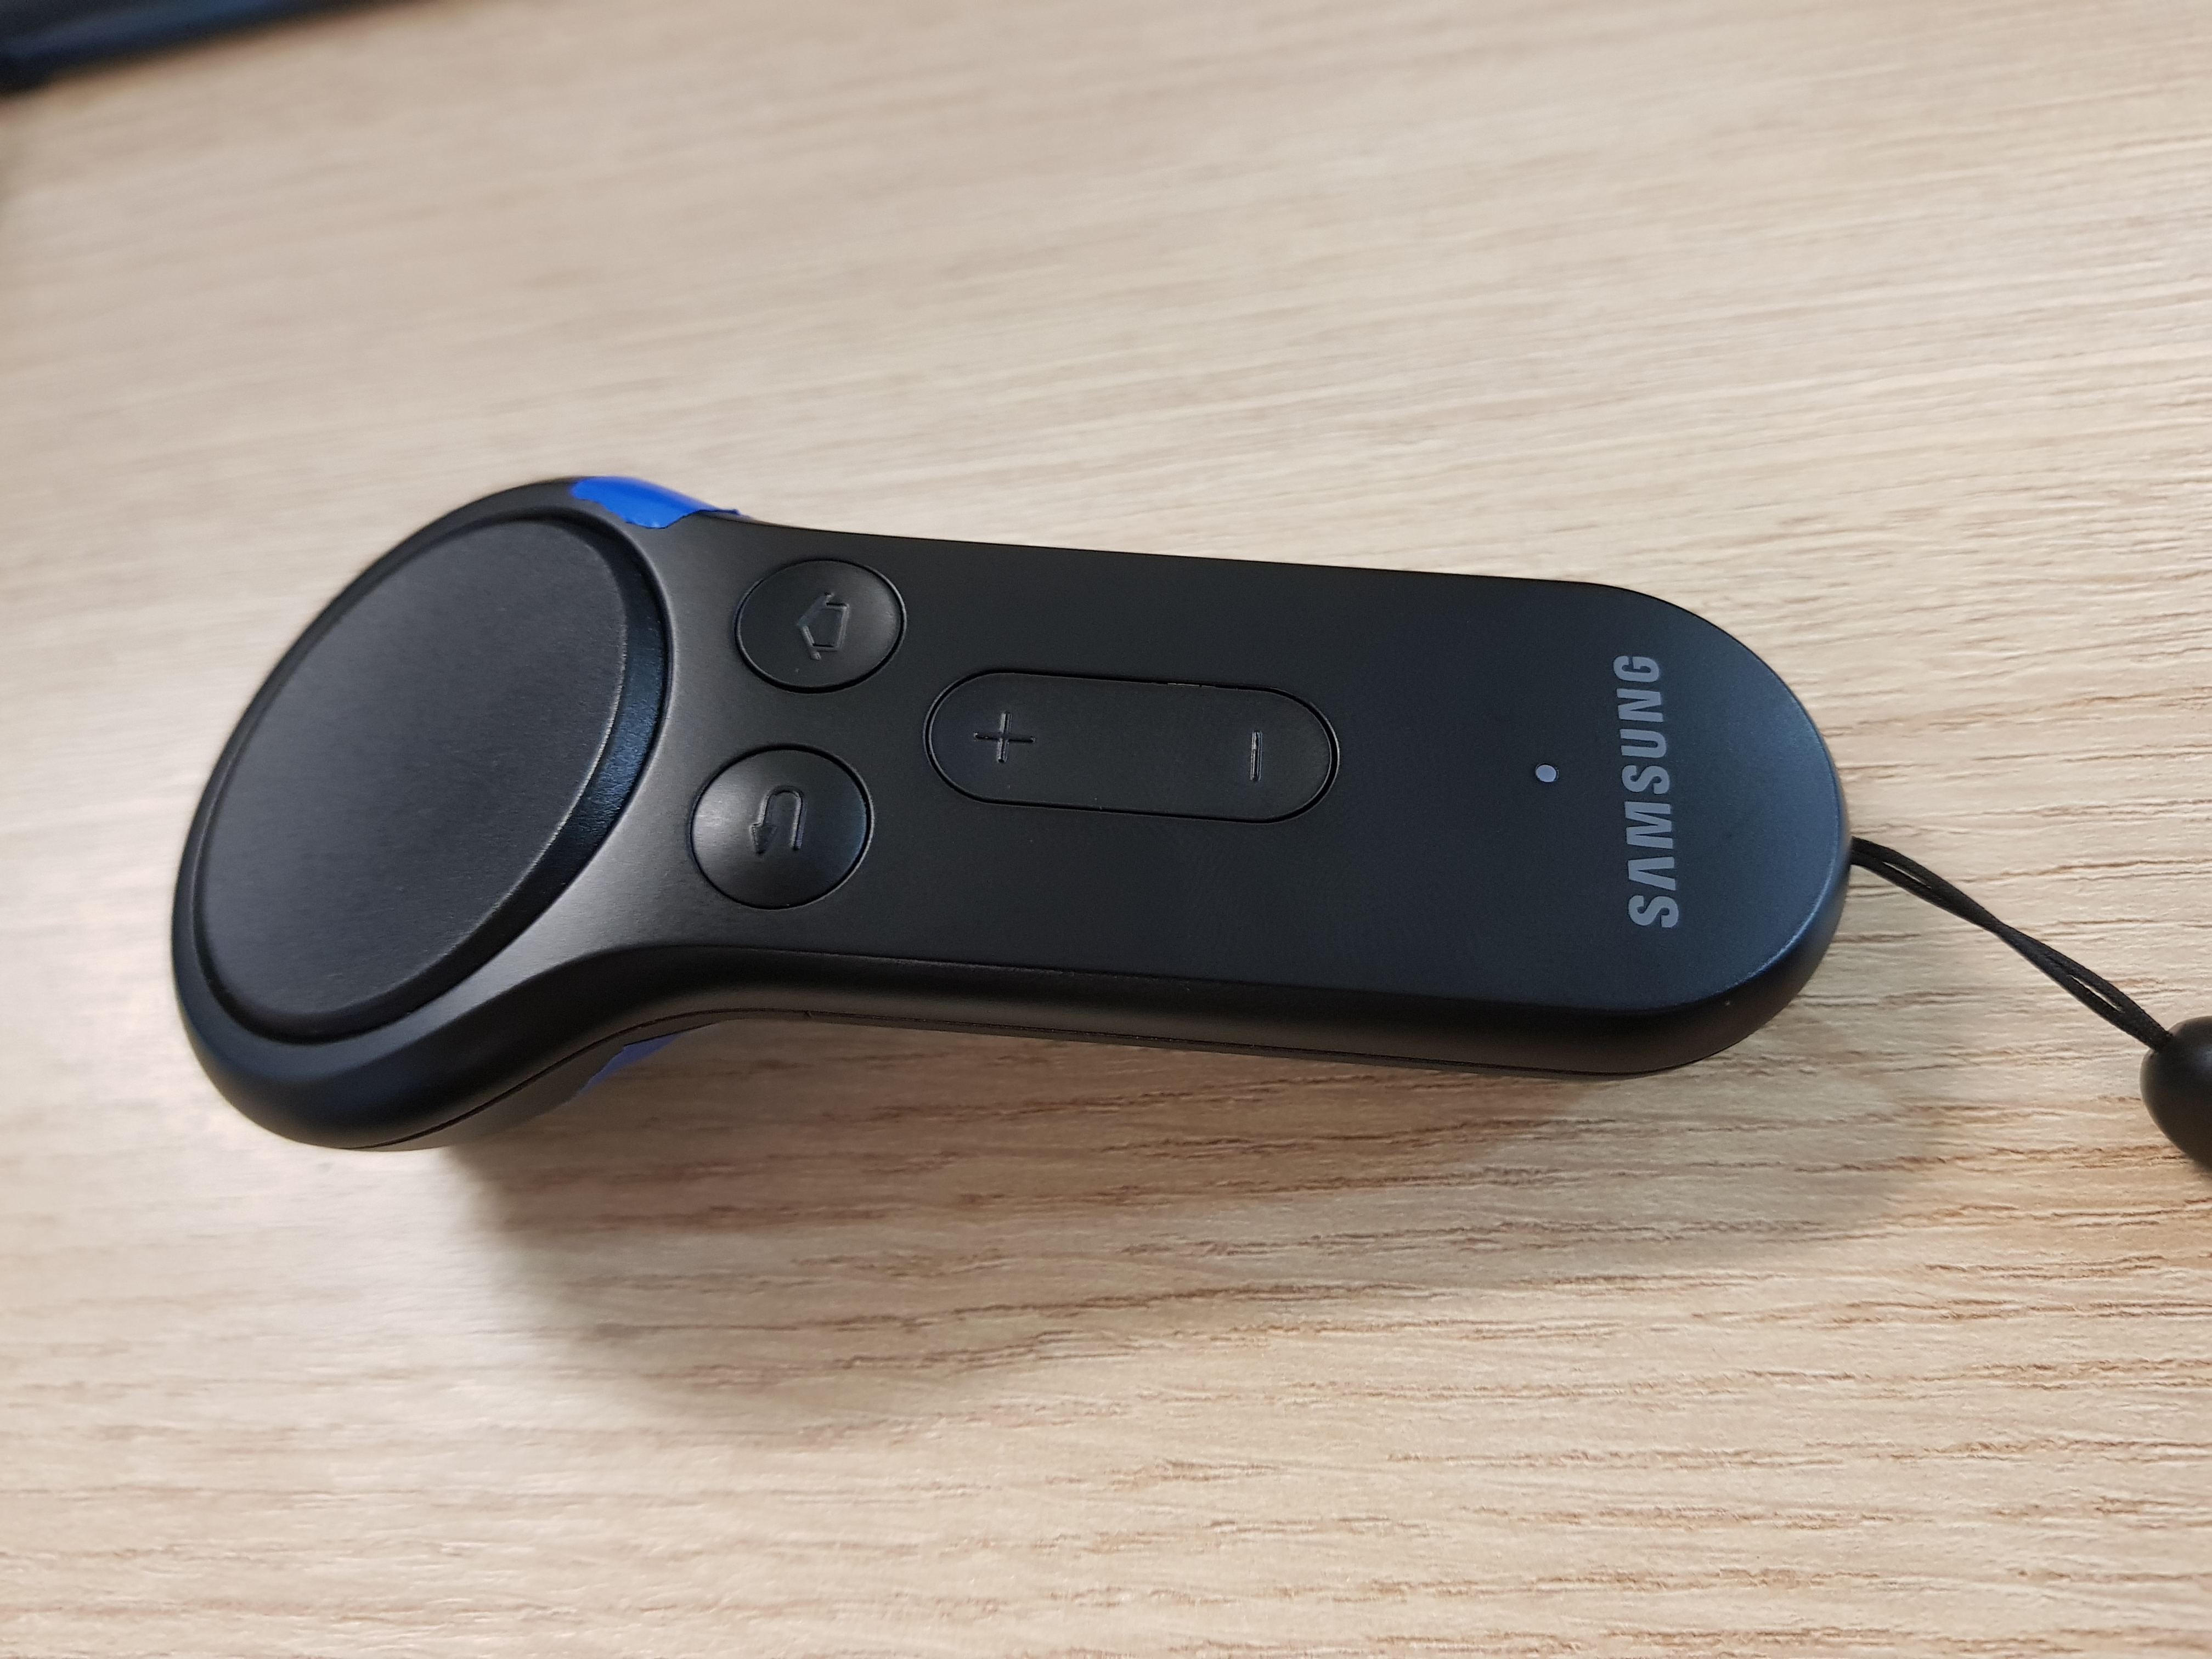
\includegraphics[width=.4\textwidth]{../images/gear_controller.jpg}
\caption{Controle para Realidade Virtual da Samsung.}
\label{fig:vrcontroller}
\end{figure}

Para a efetiva implementação do filtro de Kalman na leitura do controle de realidade virtual seguem-se os seguintes passos: inicialmente captura-se a orientação angular do \textit{joystick}, traça-se um raio da posição virtual atual do controle até uma esfera unitária e o ponto resultante da interseção é o foco do usuário, em outras palavras, o objetivo apontado pelo cursor, esta posição é onde aplica-se o filtro de Kalman, proveniente da implementação encontrada na aplicação de \cite{KalmanComponent}. O diagrama abaixo ilustra este processo.

% \begin{figure}[H]
% \centering
% \tikzstyle{rect} = [draw, rectangle, fill = white!20, text width=6em, text centered, minimum height = 4em]
% \tikzstyle{line} = [draw, -latex']

% \begin{tikzpicture} [node distance = 2cm, auto]
% \node [rect, rounded corners] (step1) {Captura da orientação angular do controle};
% \node [rect, rounded corners, right of = step1, node distance = 4cm] (step2) {Estimativa da posição do cursor};
% \node [rect, rounded corners, right of = step2, node distance = 4cm] (step3) {Aplicação do filtro de Kalman};
% %\node [rect, rounded corners, right of = step3, node distance = 4cm] (step4) {Renderização das posições ruidosas};

% \path [line] (step1) -- (step2);
% \path [line] (step2) -- (step3);
% \end{figure}

%% Geração de um cubo.

\section{Resultados} \label{sec:results}
Desenvolveu-se em realidade virtual o jogo \textit{Snake} no ambiente de desenvolvimento \textit{Unity}. Gerou-se uma aplicação \textit{android} testada no \textit{Samsung Galaxy S8} através do \textit{GearVR} com o controle de modelo ET-YO32, conforme apresentado na figura \ref{fig:vrcontroller}. A figura \ref{fig:VRPerformanceChart} abaixo ilustra a taxa de quadros no \textit{GearVR} através da ferramenta de avaliação de performance da \textit{Oculus}, o \textit{OVR Metrics Tool}:

\begin{figure}[H] \label{fig:VRPerformanceChart}
\centering
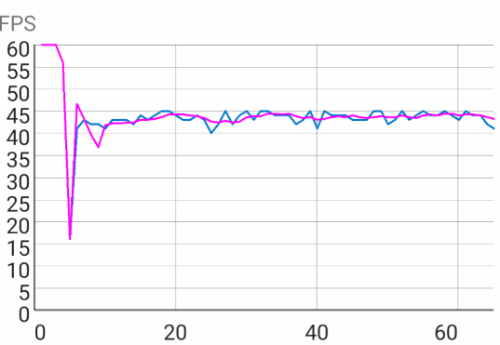
\includegraphics[scale=0.5]{VRPerformance}
\caption{Quadros-por-segundo conforme o OVR Metrics Tool executado durante o funcionamento da aplicação }
\end{figure}

A aplicação apresentou taxa média de 43.96 \textit{fps} (\textit{frames-per-second}, quadros-por-segundo), com mínima de 16 \textit{fps} e máxima de 60 \textit{fps}. Conforme representado pela figura \ref{fig:VRPerformanceChart}, a aplicação não mantém estavéis 60 \textit{fps} e isto se deve principalmente ao \textit{garbage collector} e à implementação do filtro de Kalman que, apesar de minimizar as inconsistências de leitura, ocasionou pequenos atrasos de processamento.

\section{Conclusão}\label{sec:conclusion}
% Resumo do artigo
Apresentou-se a implementação de um jogo criado segundo a arquitetura de renderização baseada em \textit{shaders} que distribui passos usualmente restritos à camada de aplicação para as demais camadas da \textit{pipeline} gráfica.

A fim de melhorar a experiência de uso do jogo com o controle, aplicou-se o filtro de Kalman com a intenção de aperfeiçoar a instabilidade presente nas leituras de movimento.

% Trabalhos Futuros
Em trabalhos futuros, três passos são percebidos como cruciais. Em primeiro lugar, migrar inteiramente os processos da camada lógica para a camada de visualização, na unidade gráfica de processamento, com o propósito de permitir o controle e exibição de um número representativamente maior de serpentes. Em segundo lugar, aplicar aprendizagem de máquina nesta camada, objetivando-se um comportamento de busca e desvio de obstáculos (como outras serpentes e seu próprio corpo) mais inteligente, por conseguinte, desafiador. Por último, otimizar e melhorar a performance, objetivando os 60 \textit{fps}.



% conference papers do not normally have an appendix


% use section* for acknowledgment
\section*{Acknowledgment}


The authors would like to thank...





% trigger a \newpage just before the given reference
% number - used to balance the columns on the last page
% adjust value as needed - may need to be readjusted if
% the document is modified later
%\IEEEtriggeratref{8}
% The "triggered" command can be changed if desired:
%\IEEEtriggercmd{\enlargethispage{-5in}}

% references section

% can use a bibliography generated by BibTeX as a .bbl file
% BibTeX documentation can be easily obtained at:
% http://mirror.ctan.org/biblio/bibtex/contrib/doc/
% The IEEEtran BibTeX style support page is at:
% http://www.michaelshell.org/tex/ieeetran/bibtex/
%\bibliographystyle{IEEEtran}
% argument is your BibTeX string definitions and bibliography database(s)
%\bibliography{IEEEabrv,../bib/paper}
%
% <OR> manually copy in the resultant .bbl file
% set second argument of \begin to the number of references
% (used to reserve space for the reference number labels box)
\bibliographystyle{IEEEtran}

% \bibliographystyle{ieeetran}
\bibliography{bare_conf}




% that's all folks
\end{document}


